\section{3. Modulaci\'on de se\~nal con AM}
Para la siguiente secci\'on se emplearon dos generadores, uno para generar la señal portadora y otro para la moduladora. La frecuencia de la portadora fue de $800kHz$ y la de la moduladora de $100Hz$. Se cre\'o una señal modulada en amplitud fijando el factor de modulaci\'on $m$ y variando la aplitud de la señal portadora hasta conseguir $250mV_{pp}$ medidos a la entrada del analizador de espectros. Se tomaron cuatro mediciones diferentes: moduladora senoidal con $m = 0.5$ y $m = 1$, moduladora triangular con $m = 1$ y moduladora senoidal con $m = 1$ y frecuencia igual a la portadora.

\subsection{Mediciones}

A continuaci\'on se muestran las capturas de pantalla del analizador de espectros con sus respectivos gráficos teóricos:

\begin{figure}[H]
    \centering
    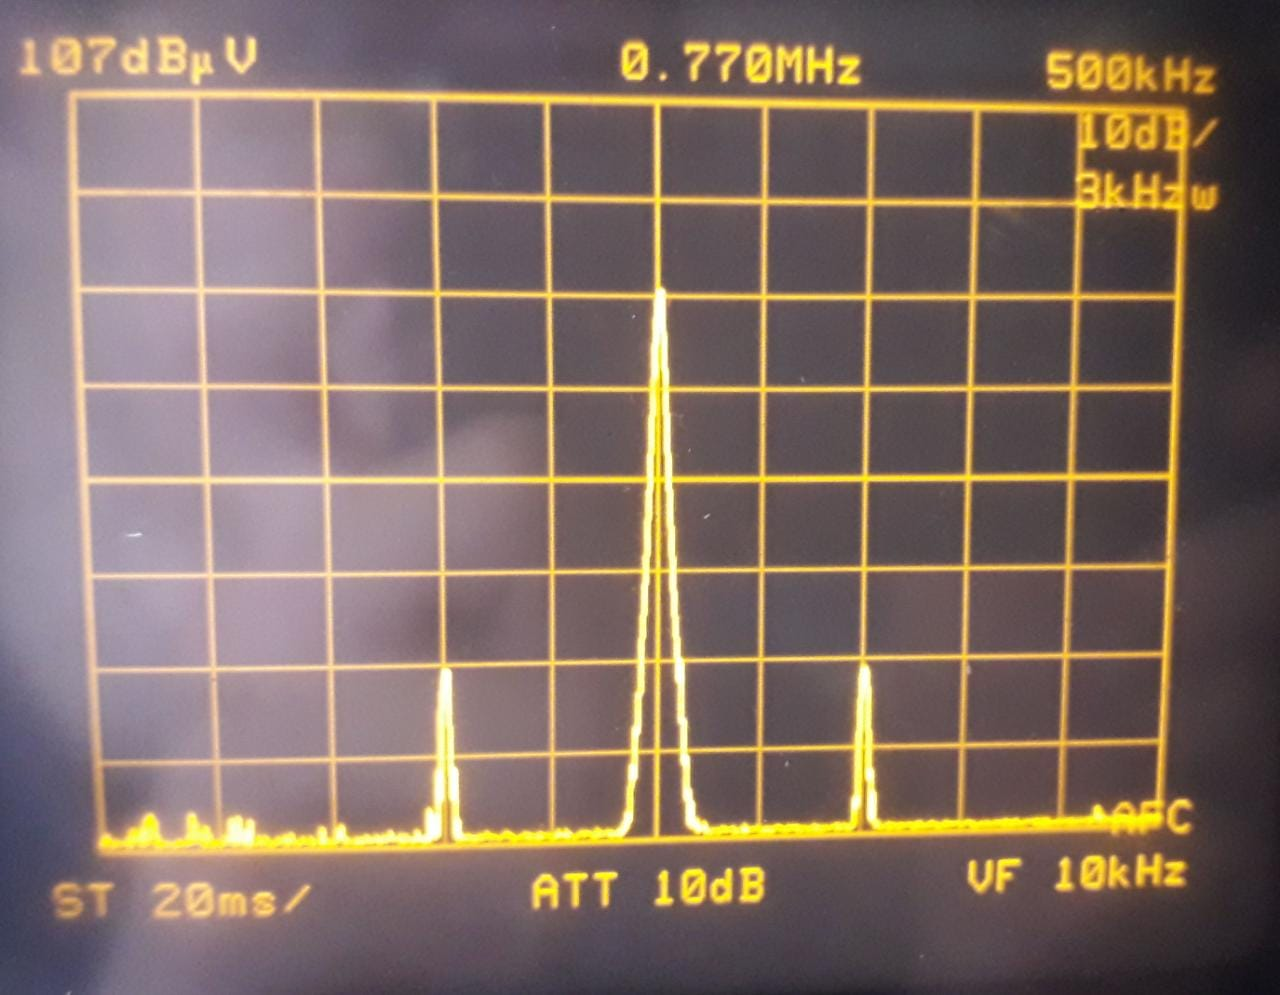
\includegraphics[scale=0.3]{Recursos/Ej3_senoidal_m05.jpeg}
    \caption{Espectro señal senoidal con $m = 0.5$}
\end{figure}

\begin{figure}[H]
    \centering
    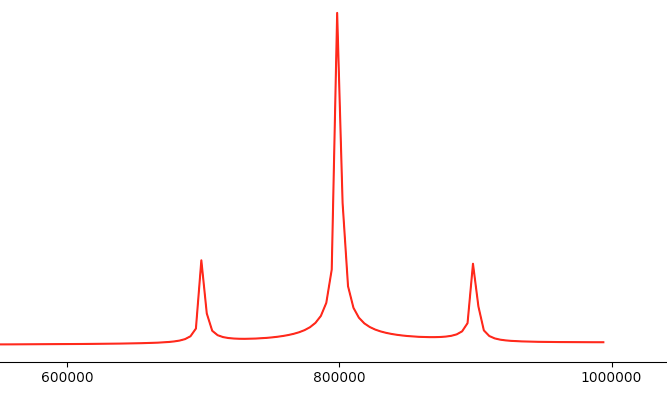
\includegraphics[scale=0.5]{Recursos/Ej3_senoidal_m05_teorico.png}
    \caption{Espectro señal senoidal con $m = 0.5$ teórica}
\end{figure}

\begin{figure}[H]
    \centering
    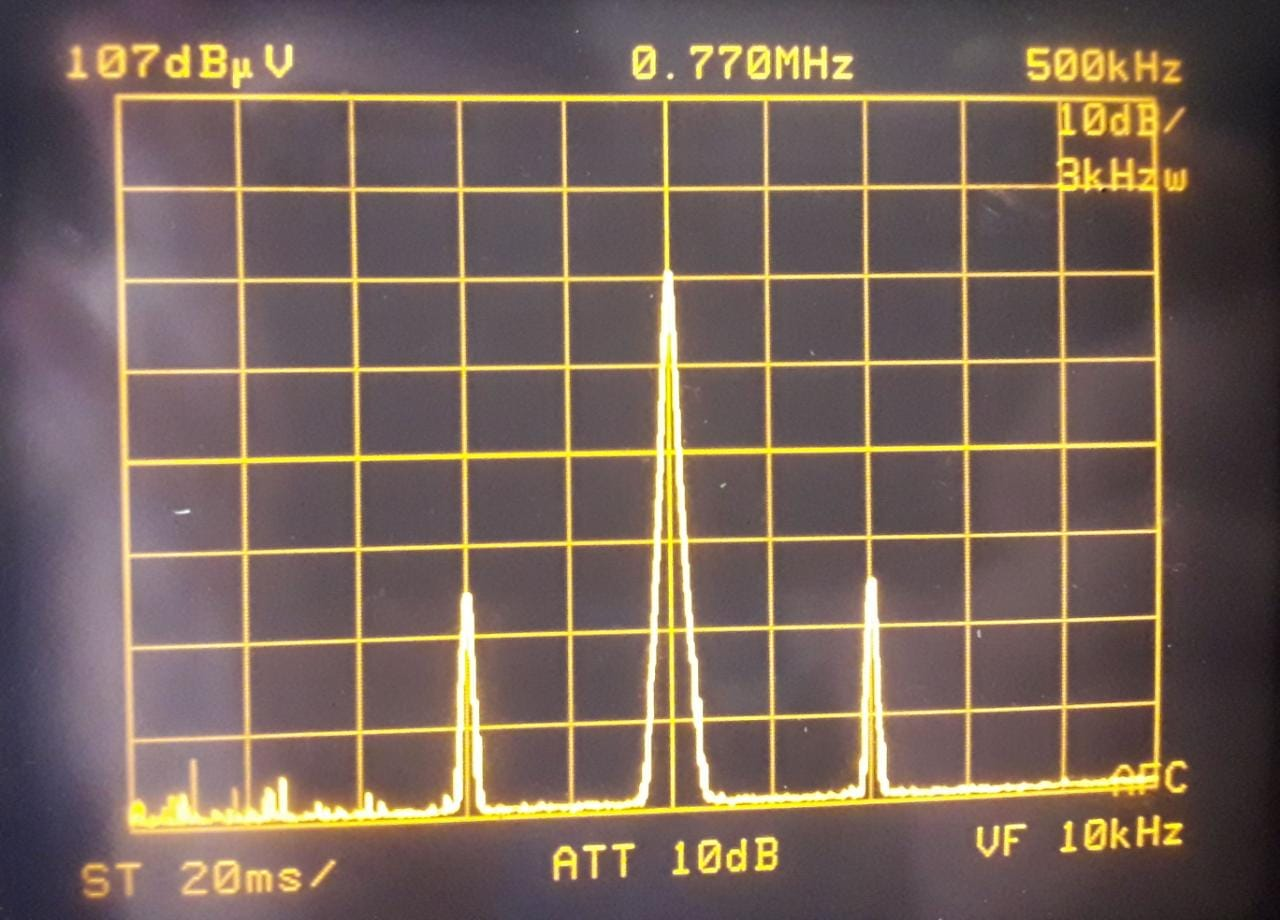
\includegraphics[scale=0.3]{Recursos/Ej3_senoidal_m1.jpeg}
    \caption{Espectro señal senoidal con $m = 1$}
\end{figure}

\begin{figure}[H]
    \centering
    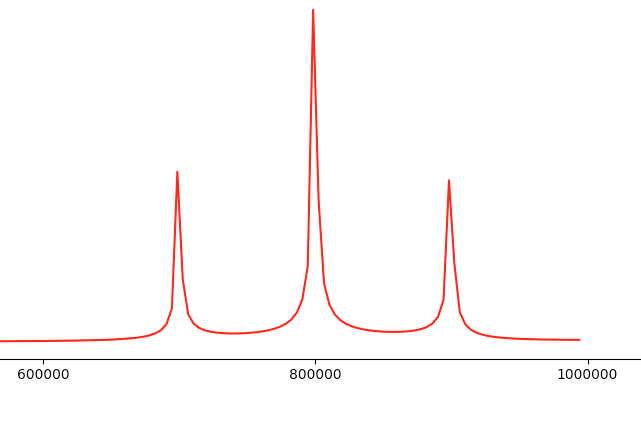
\includegraphics[scale=0.5]{Recursos/Ej3_senoidal_m1_teorico.png}
    \caption{Espectro señal senoidal con $m = 1$ teórica}
\end{figure}

\begin{figure}[H]
    \centering
    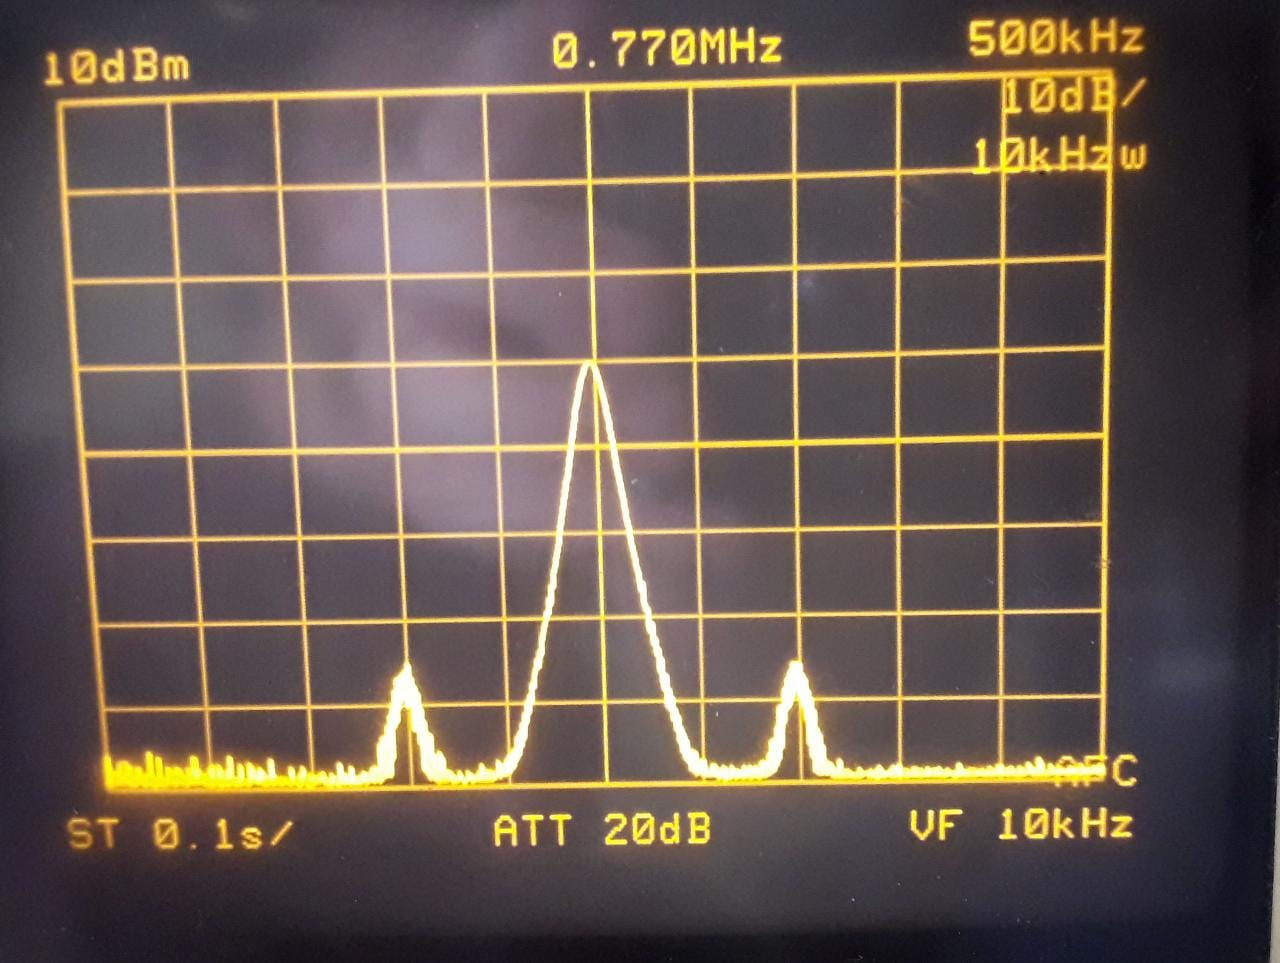
\includegraphics[scale=0.3]{Recursos/Ej3_triangular_m1.jpeg}
    \caption{Espectro señal triangular con $m = 1$}
\end{figure}\label{fig:triangular_ej3}

\begin{figure}[H]
    \centering
    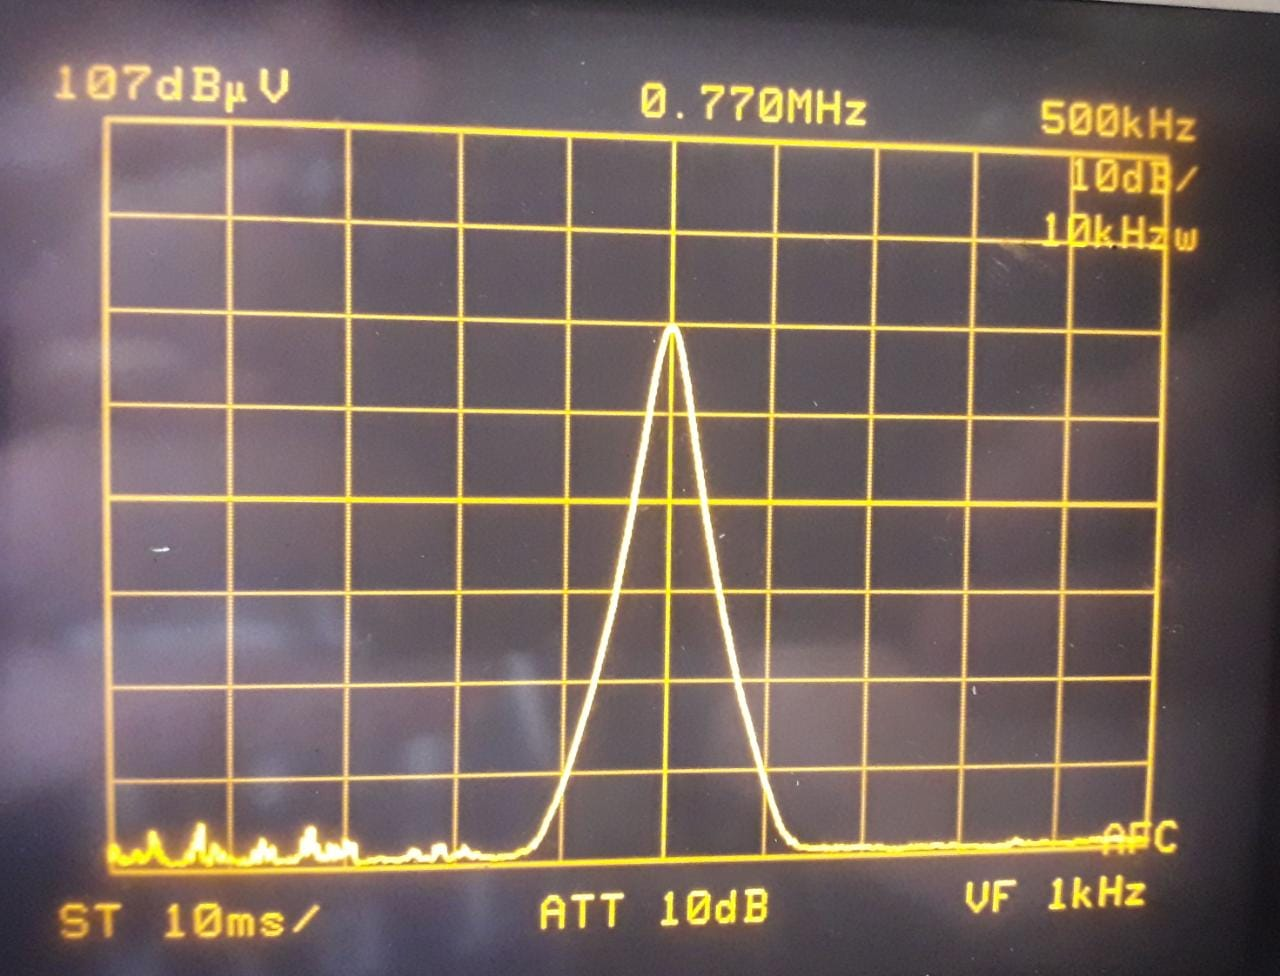
\includegraphics[scale=0.3]{Recursos/Ej3_senoidal_800K.jpeg}
    \caption{Espectro señal senoidal con frecuenca de portadora}
\end{figure}

\begin{figure}[H]
    \centering
    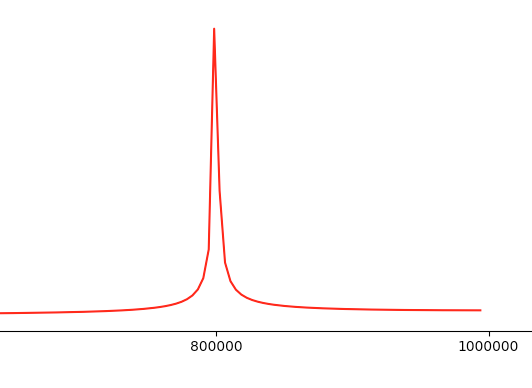
\includegraphics[scale=0.5]{Recursos/Ej3_senoidal_igualf_teorico.png}
    \caption{Espectro señal senoidal con frecuenca de portadora teórica}
\end{figure}

\subsection{An\'alisis de los resultados}

En primer lugar todas las mediciones concuerdan en forma con las simulaciones correspondientes. La única diferencia que existe es con la precisión de la frecuencia de la portadora, la cuál se observó corrida en $30kHz$ respecto al valor teórico.\newline

El espectro de las dos primeras figuras revela que existen dos bandas-laterales, a cada lado de la frecuencia portadora. Lo anterior surge de la interferencia entre las frecuencias de la portadora y la modulante. Como resultado se obtiene la suma y la diferencia entre ambas frecuencias. Debido a que el factor de modulaci\'on es mayor para la segunda figura, las bandas laterales aparecen menos atenuadas. Debido que para el caso $d$ las frecuencias eran id\'enticas, no se observan las bandas laterales. Por \'ultimo, para la señal triangular tambi\'en se observan las bandas laterales, pero adem\'as se ve una banda de frecuencias al rededor de la frecuencia fundamental. Como se expic\'o en el ejercicio anterior, la señal triangular puede escribirse como una suma infinita de arm\'onicos . Pero la mayor parte de la potencia de la señal ($x\%$), corresponde a los primeros 5 arm\'onicos. Por esta raz\'on , en lugar de verse una \'unica frecuencia se ve una banda y los dem\'as arm\'onicos no se distinguen del piso de ruido.




